\documentclass[11pt]{article}

\usepackage{arxiv}

\usepackage[utf8]{inputenc}
\usepackage{amsmath, amssymb}
\usepackage{graphicx}
\usepackage{listings}
\usepackage{color}
\usepackage{caption}
\usepackage{float}

\title{TP2.2 - Generadores de números pseudoaleatorios de distintas Distribuciones de Probabilidad.}

\author{
 Pecoraro Lucio \\
  Universidad Tecnológica Nacional - FRRO\\
  Zeballos 1341, S2000, Argentina\\
  Legajo 50239 \\
  \texttt{luciopecoraro2002@gmail.com} \\
  %% examples of more authors
   \And
 Berto Leandro \\
  Universidad Tecnológica Nacional - FRRO\\
  Zeballos 1341, S2000, Argentina\\
  Legajo 45368 \\
  \texttt{leandroberto2010@gmail.com} \\
  \And
 Capiglioni Rodrigo \\
  Universidad Tecnológica Nacional - FRRO\\
  Zeballos 1341, S2000, Argentina\\
  Legajo 47298 \\
  \texttt{RodrigoCapiglioni@gmail.com} \\
  \And
  Broda Tomás \\
  Universidad Tecnológica Nacional - FRRO\\
  Zeballos 1341, S2000, Argentina\\
  Legajo 47299 \\
  \texttt{tomasbroda13@gmail.com} \\
  }

  % Estilo para código Python
\definecolor{codegray}{gray}{0.9}
\lstset{
  backgroundcolor=\color{codegray},
  basicstyle=\ttfamily\small,
  frame=single,
  language=Python,
  keywordstyle=\color{blue},
  commentstyle=\color{green!50!black},
  numbers=left,
  numberstyle=\tiny,
  breaklines=true,
  showstringspaces=false
}

\begin{document}
\maketitle

\begin{abstract}
Este trabajo tiene como propósito analizar diversas distribuciones de probabilidad, detallando sus principales características. Se abordará el desarrollo conceptual de cada una, se empleará tecnología para ilustrar su comportamiento y, finalmente, se evaluará la generación de valores a través de pruebas específicas\end{abstract}

\section{Introducción}
Se busca analizar cómo se generan distintos tipos de distribuciones mediante la producción de números pseudoaleatorios. Se trabajará con distribuciones tanto continuas como discretas, utilizando generadores específicos para cada caso. Tras llevar a cabo las simulaciones, se aplicará la prueba de bondad de ajuste Chi-Cuadrado en algunos de los conjuntos de datos obtenidos para evaluar sus resultados.

\section{Distribuciones de Probabilidad}
En teoría de la probabilidad y estadística, la distribución de probabilidad de una variable aleatoria es una función que asigna a cada suceso definido sobre la variable aleatoria, la probabilidad de que dicho suceso ocurra. La distribución de probabilidad está definida sobre el conjunto de todos el rango de valores de la variable aleatoria.

La distribución de probabilidad está completamente especificada por la función de distribución, cuyo valor en cada x real es la probabilidad de que la variable aleatoria sea menor o igual que x. Los tipos de variables existentes son:

\begin{itemize}
    \item\textbf{Variable aleatoria:} Es aquella cuyo valor es el resultado de un evento aleatorio. Lo que quiere decir que son los resultados que se presentan al azar en cualquier evento o experimento.
    \item\textbf{Variable aleatoria discreta:} Es aquella que solo toma ciertos valores (frecuentemente enteros) y que resulta principalmente del conteo realizado.
    \item\textbf{Variable aleatoria continua:} Es aquella que resulta generalmente de la medición y puede tomar cualquier valor dentro de un intervalo dado.

\end{itemize}

A continuación se desarrollarán distintos generadores de valores de variables aleatorias a partir de las distribuciones probabilidad, las cuales están clasificadas según el tipo de variable.


\subsection{Distribuciones Continuas de Probabilidad}
  Una distribución continua describe las probabilidades de los posibles valores de una variable aleatoria continua. Una variable aleatoria continua es una variable aleatoria con un conjunto de valores posibles (conocido como el rango) que es infinito y no se puede contar.

\subsubsection{Distribución Uniforme}
  Se distingue por su constancia dentro de un intervalo definido entre ( a ) y ( b ), excluyendo el valor cero. Su origen radica en el análisis de los errores de redondeo al registrar mediciones con un determinado nivel de precisión. Se destaca frente a otros métodos de simulación debido a su simplicidad y versatilidad, ya que permite modelar variables aleatorias basadas en prácticamente cualquier distribución de probabilidad.


\noindent\textbf{Función de Densidad}\\
Describe una variable aleatoria continua en la que todos los valores dentro de un intervalo tienen la misma probabilidad de ocurrir
\[
f(x) = 
\begin{cases}
\frac{1}{b - a}, & a \leq x \leq b \\
0, & \text{en otro caso}
\end{cases}
\]

\noindent\textbf{Función Acumulada}\\
Representa la probabilidad acumulada desde el valor mínimo hasta el valor dado
\[
F(x) = 
\begin{cases}
0, & x < a \\
\frac{x - a}{b - a}, & a \leq x \leq b \\
1, & x > b
\end{cases}
\]
En esta ecuación  X es una variable aleatoria definida en (a, b). El valor esperado y la varianza de una variable aleatoria uniformemente distribuida, se puede representar por:
  \begin{equation}
    EX = \frac{b+a}{2}
  \end{equation}
  \begin{equation}
    VX = \frac{(b-a)^2}{12}
  \end{equation}

\noindent\textbf{Método de la transformación inversa}\\
  Para simular una distribución uniforme sobre cierto intervalo conocido (a,b) deberemos, en primer lugar, obtener la transformación inversa para la distribución uniforme acumulativa:
\begin{equation}
    F(x) = \int_{0}^{a}\frac{1}{b-a}dt = \frac{x-a}{b-a} \ \text{  } \ 0 \leq F(x) \leq 1.
  \end{equation}
Lo cual podemos deducir como su función inversa a:
  \begin{equation}
  x = a +(b-a)r \ \text{  }\ 0 \leq r \leq 1.
  \end{equation}
En seguida, generamos un conjunto de números aleatorios correspondientes al rango de las probabilidades acumulativas, es decir, los valores de variables aleatorias uniformes definidas sobre el rango 0 a 1. Cada número aleatorio r determina, de manera única, un valor de la variable x uniformemente distribuida.
\newpage
\noindent\textbf{Código en Python}

\begin{lstlisting}
import random
import math

def distr_uniforme(a, b, size):
    x=[]
    for _ in range(size):
        x.append(a+(b-a)*random.random())
    return x

def uniforme_rechazo(a,b):
    while True:
        r1 = random.uniform(0,1)
        X = a + (b - a) * r1
        c = 1 / (b - a)
        r2 = random.uniform(0,1) 
        if r2 <= c :
            return X
    
\end{lstlisting}
Se ingresa como parámetro a y b que son valores que expresan los límites de las distribuciones uniformes.

\noindent\textbf{Gráfico}

\begin{center}
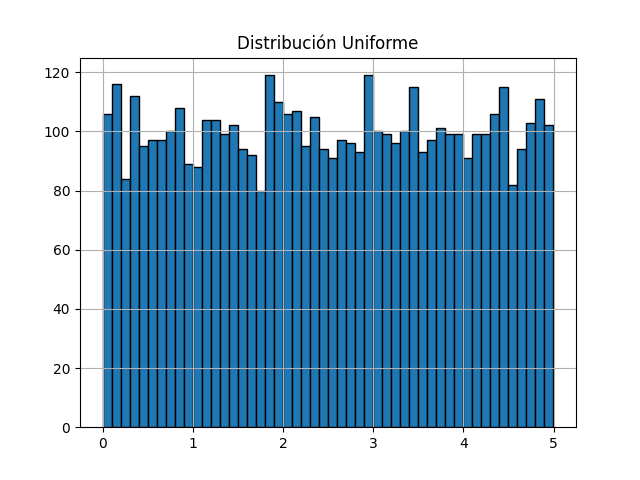
\includegraphics[width=0.7\textwidth]{histograma_uniforme.png}
\captionof{figure}{Histograma para la distribución uniforme continua \( U(5,15) \).}
\end{center}


\newpage

\subsubsection{Distribución Exponencial}

Si un evento ocurre dentro de intervalos cortos de manera independiente de otros eventos, el tiempo transcurrido entre sucesos sigue una distribución exponencial.
\paragraph*{Función de Densidad\newline}
\[
f(x) = 
\begin{cases}
\lambda e^{-\lambda x}, & x \geq 0 \\
0, & x < 0
\end{cases}
\]

\noindent\textbf{Función Acumulada}\\
\[
F(x) = 1 - e^{-\lambda x}
\]
y la media junto con la variancia de X se pueden expresar como
  \begin{equation}
    EX = \int_{0}^{\infty} xae^{-ax}dx = \frac{1}{a}
  \end{equation}
  \begin{equation}
  VX = \int_{0}^{\infty} (x-\frac{1}{a})^2 = \frac{1}{a^2} = (EX)^2
\end{equation}
  
\noindent\textbf{Método de la transformación inversa}\\

Existen muchas maneras para lograr la generación de valores de variables aleatorias exponenciales. Puesto que la distribución acumulativa existe explícitamente (vista en la ecuación (8)),la técnica de la transformación inversa nos permite desarrollar métodos directos para dicha generación.
Debido a la simetría que existe entre la distribución uniforme sigue que la intercambiabilidad de F(x) y 1 - F(x). Por lo tanto:
\begin{equation}
r = e^{-\lambda x}
\end{equation}
y consecuentemente
\begin{equation}
x = -\frac{1}{\lambda}log r  = - EXlog r
\end{equation}
Por consiguiente, para cada valor del número pseudoaleatorio \( r \), se determina un único valor para \( x \). Los valores de \( x \) toman tan sólo magnitudes no negativas, debido a que \( \log(r) \leq 0 \) para \( 0 \leq r \leq 1 \), y además se ajustan a la función de densidad exponencial con un valor esperado \( x \). Es importante notar que, pese a que esta técnica parece en principio muy simple, es preciso recordar que en una computadora digital el cálculo logarítmico natural involucra una expansión en serie de potencias para cada valor de la variable aleatoria que se debe generar.

\newpage
\noindent\textbf{Gráfico}

\begin{center}
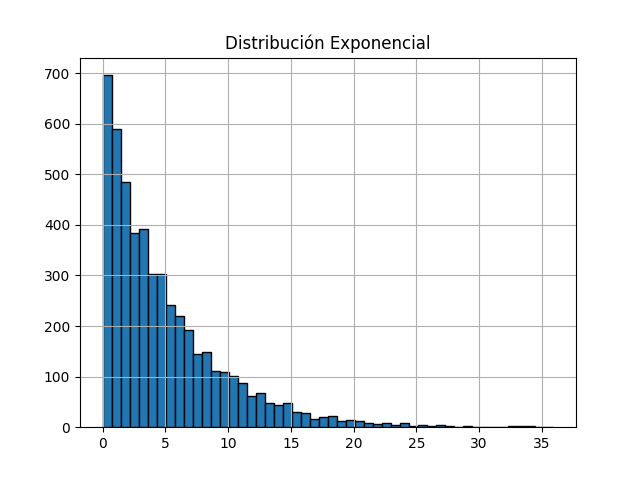
\includegraphics[width=0.7\textwidth]{histograma_exponencial.png}
\captionof{figure}{Histograma para la distribución uniforme continua \( U(5,15) \).}
\end{center}



\subsubsection{Distribución Gamma}
Si un determinado proceso está compuesto por k eventos que ocurren de manera sucesiva, y si el tiempo total del proceso puede modelarse como la suma de k variables aleatorias independientes, donde cada una sigue una distribución exponencial con el mismo parámetro, entonces la variable que representa el tiempo total sigue una distribución gamma con parámetros a y k. \\
\\
\noindent\textbf{Función de Densidad}\\
La función gamma está descrita mediante la siguiente función de densidad:
  \begin{equation}
    f(x) = \frac{a^{k}x^{(k-1)}e^{-ax}}{(k-1)!}
  \end{equation}
  donde $a > 0  ,  k > 9$ y x se considera no negativo.
  Respecto a la media y la variancia de esta distribución, sus corrspondientes expresiones están formuladas como sigue:
  \begin{equation}
    EX = \frac{k}{a}
  \end{equation}
  \begin{equation}
    VX = \frac{k}{a^{x}}
  \end{equation}

\newpage
\noindent\textbf{Gráfico}\\
\begin{figure}[h]
    \centering
    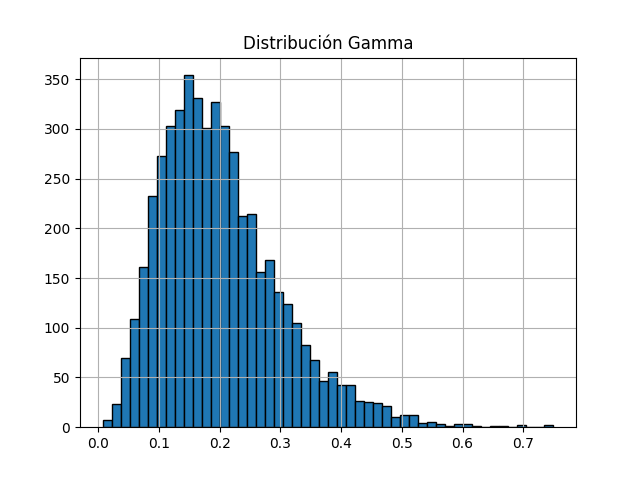
\includegraphics[width=0.6\textwidth]{histograma_gamma.png}
    \caption{Frecuencias absolutas de valores generados.}
  \end{figure}

\subsubsection{Distribución Normal}
La distribución normal basa su utilidad en el teorema del límite central. Este postula que la distribución de probabilidad de la suma de \( N \) valores de una variable aleatoria \( x \), independientes pero idénticamente distribuidos, con medias respectivas \( \mu \) y varianzas \( \sigma^2 \), se aproxima asintóticamente a una distribución normal a medida que \( N \) se hace muy grande.


En consecuencia, el teorema del límite central permite el empleo de distribuciones normales para representar medidas globales operadas sobre los efectos de causas (errores) aditivas distribuidas en forma independiente sin importar la distribución de probabilidad a que obedezcan las mediciones de causas individuales. 

\noindent\textbf{Función de Densidad}\\
Si la variable aleatoria X tiene una función de densidad f(x) dada como:
\begin{equation}
f(x) = \frac{1}{\sigma_{x}\sqrt{2\pi}} e^{\frac{-(x - \mu)^2}{2\sigma^2}}
\end{equation}

El valor esperado y la variancia de la distribución normal están dados por:
  \begin{equation}
    EX = \mu_{x}
  \end{equation}
  \begin{equation}
    EX = \sigma_{x}^2
  \end{equation}

\noindent\textbf{Método de la transformación inversa\newline}
  El procedimiento para simular valores normales utilizando computadoras requiere el uso de la suma de K valores de
  variables aleatorias distribuidos uniformemente; esto es la suma de r1, r2... rk con cada ri definida en el intervalo $0 <  ri <  1$. Aplicando la convención notacional de la forma matemática del teorema central del límite, encontramos que:
  \begin{equation}
    \theta = \frac{a+b}{2} = \frac{0+1}{2} = \frac{1}{2},
  \end{equation}
  \begin{equation}
    \sigma = \frac{b-a}{\sqrt {12}} = \frac{1}{\sqrt {12}},
  \end{equation}
  \begin{equation}
    z = \frac{\sum_{i=2}^{K}r_{i}-K/2}{\sqrt {K/12}}
  \end{equation}
  Pero por definición, z es un valor de variable aleatoria con distribución normal estándar.
  Por lo tanto:

  \begin{equation}
    x = \sigma_{x}(\frac{12}{K})^{1/2}(\sum_{i=1}^{K}r_{i}-\frac{K}{2}) + \mu_{x}
  \end{equation}
  Por lo tanto, con la ecuación anterior, podemos proporcionar una formulación muy simple para generar valores de
  variable aleatoria normalmente distribuidos. Para generar un solo valor x bastará con sumar K números aleatorios
  definidos en el intervalo de 0 a 1. Este procedimiento se puede repetir tantas veces como valores de variables aleatorias
  normalmente distribuidos se quieran

\noindent\textbf{Código en Python}\\

\begin{lstlisting}
import random
import math

def distr_normal(ex, stdx, size):
    x=[]
    for _ in range(size):
        sum=0
        for _ in range(12):
            sum=sum+random.random()
        x.append(stdx*(sum-6)+ex)
    return x

def normal_rechazo(mu, sigma):
    while True:
        r1 = random.uniform(0,1)
        r2 = random.uniform(0,1)
        Z = math.sqrt(-2*math.log(r1))* math.cos(2*math.pi*r2)
        X = Z * sigma + mu 
        c = math.exp(-0.5*((X-mu)/sigma)**2)/(sigma*math.sqrt(2*math.pi))
        r = random.uniform(0,1)
        if r <= c :
            return X
\end{lstlisting}
Se puede observar que se ingresa como parámetro la media ex y la desviación estándar que es stdx.

\noindent\textbf{Gráfico}\\

\begin{center}
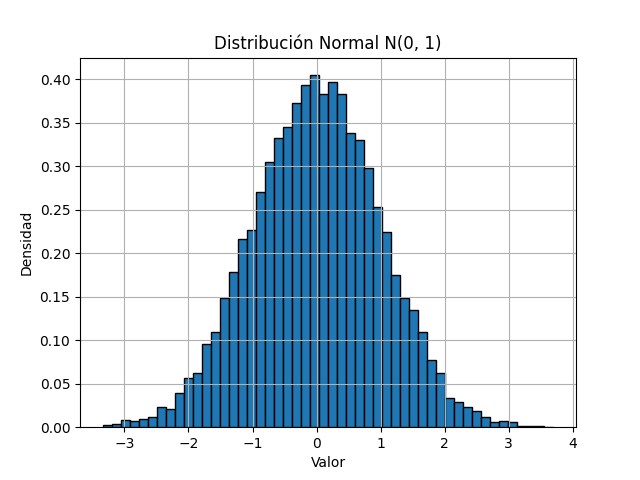
\includegraphics[width=0.7\textwidth]{histograma_normal.png}
\captionof{figure}{Histograma para la distribución normal.}
\end{center}


\subsection{Distribuciones Discretas de Probabilidad}
Se encuentra definido un número muy significativo de distribuciones de probabilidad para variables aleatorias que solamente toman valores discretos, esto es, enteros no negativos. La distribución acumulativa de probabilidad para una variable aleatoria discreta X se define de manera muy similar a la de la ecuación
\begin{equation}
F(x) = P(X \leq x) = \sum_{x=0}^{x}f(x)
\end{equation}
Donde f(x) es la frecuencia o función de probabilidad de X definida por valores enteros que:
\begin{equation}
F(x) = P(X= x)
\end{equation}
Para x=0,1,2,...
Las distribuciones discretas de probabilidad son muy útiles cuando se las emplea como modelos estocásticos para ciertos procesos de conteo, ya sea sobre muestras finitas o no finitas, donde la presencia o ausencia de un atributo dicotómico está gobernada por el azar.

Las secciones siguientes contienen la descripción de técnicas para la generación de valores de variables estocásticas a partir de la mayoría de las distribuciones discretas de p

\subsubsection{Distribución de Pascal}
La variable aleatoria de Pascal es una extensión de la variable aleatoria geométrica. Describe el número de ensayos hasta el tiempo entre llegadas de un proceso de Bernoulli. La distribución de Pascal también se denomina distribución binomial negativa.
\\ \\
\noindent\textbf{Función de Probabilidad\newline}
Sea $X_k$ una variable aleatoria de Pascal de orden k:
 \begin{equation}
    P(X = x) = (\frac{k+x-1}{x})p^{k}q^{x} \ \text{   } \ x = 0,1,2,...,
  \end{equation}
  donde k es el número total de éxitos en una sucesión de k + x ensayos, con x el número de fallas que ocurren antes de obtener k éxitos.

  El valor esperado y la variancia de X se representa con:

  \begin{equation}
    EX = \frac{kq}{p}
  \end{equation}
  \begin{equation}
    VX = \frac{kq}{p^2}
  \end{equation}

\noindent\textbf{Gráfico\newline}
\begin{center}
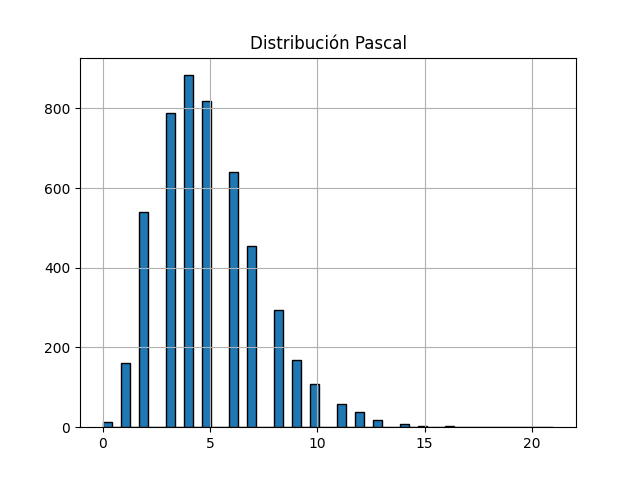
\includegraphics[width=0.7\textwidth]{histograma_pascal.png}
\captionof{figure}{Histograma para la distribución pascal.}
\end{center}
  

\subsubsection{Distribución Binomial}
La distribución binomial modela la probabilidad de obtener exactamente x éxitos en n ensayos de Bernoulli independientes, donde cada ensayo tiene una probabilidad de éxito p.

\noindent\textbf{Funcion de Probabilidad\newline}
\[
P(X = x) = \binom{n}{x} p^x (1 - p)^{n - x}, \quad x = 0, 1, 2, \dots, n
\]
\begin{itemize}
    \item n: número de ensayos.
    \item x: número de éxitos.
    \item p: probabilidad de éxito en cada ensayo. 
    \item ($\frac{n}{x}$): coeficiente binomial (combinaciones de n elementos tomados de a x).
\end{itemize}
La esperanza y la variancia se definen de la siguiente manera:
\[
\mathbb{E}[X] = np, \quad \text{Var}(X) = np(1 - p)
\]

\noindent\textbf{Gráfico\newline}
\begin{center}
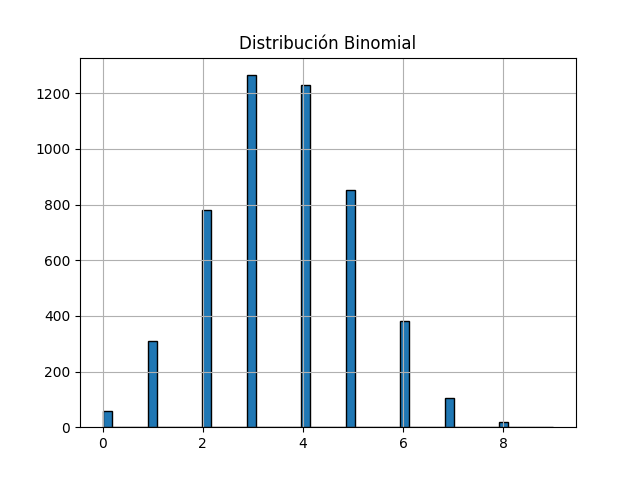
\includegraphics[width=0.7\textwidth]{histograma_binomial.png}
\captionof{figure}{Histograma para la distribución binomial.}
\end{center}

\subsubsection{Distribución Hipergeométrica}
Modela la cantidad de éxitos al extraer una muestra sin reemplazo de tamaño n desde una población de tamaño N, que contiene K elementos exitosos.

La función de probabilidad de una variable aleatoria con distribución hipergeométrica puede deducirse a través de razonamientos combinatorios y es igual a:
\begin{equation}
    f(x) = \frac{\binom{N_{p}}{x}\binom{N_{q}}{n-x}}{\binom{N}{n}}
    \end{equation}
  con $0 =< x =< Np$, y $0 =< n-x =<Nq$. Donde x,n y N son enteros. El valor esperado y la variancia se caracterizan como sigue:
  \begin{equation}
    EX = np
    \end{equation}

  \begin{equation}
    VX = npq(\frac{N-n}{N-1})
    \end{equation}
  La generación de valores hipergeométricos involucra, substancialmente, la simulación de experimentos de muestreo sin reemplazo.


\subsubsection{Distribución Poisson}
Modela la cantidad de eventos que ocurren en un intervalo de tiempo o espacio bajo una tasa de ocurrencia constante \( \lambda \).
 Si tomamos una serie de n ensayos independientes de Bernoulli, en cada uno de los cuales se tenga una probabilidad p muy pequeña relativa a la ocurrencia de un cierto evento,
  a medida que n tiende al infinito, la probabilidad de x ocurrencias está dada por la distribución de Poisson
  \begin{equation}
    f(x) = \frac{e^{-\lambda} \lambda^k}{k!}, \quad k = 0, 1, 2, \ldots
    \end{equation}
Esto sucede siempre y cuando permitamos que p se aproxime a cero de manera que se satisfaga la relación \(\ \lambda = np. \)\

\noindent\textbf{Gráfico\newline}
\begin{center}
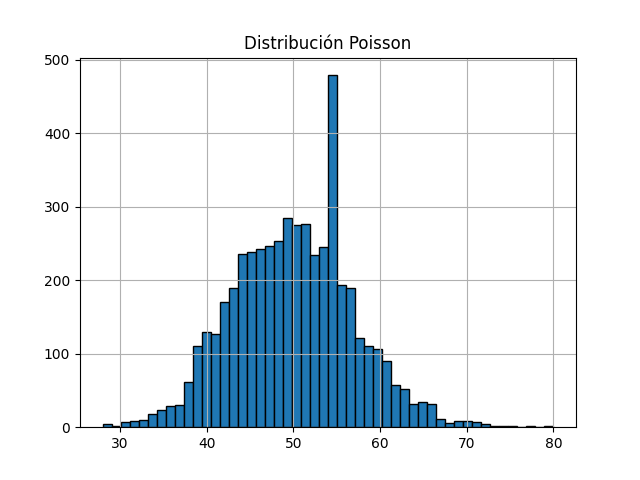
\includegraphics[width=0.7\textwidth]{histograma_poisson.png}
\captionof{figure}{Histograma para la distribución Poisson obtenida.}
\end{center}

\subsubsection{Distribución Empírica Discreta}
Sea \( X \) una variable aleatoria discreta tal que \( P(X = b_i) = p_i \).  
Una forma directa de generar esta variable en una computadora consiste en utilizar un número aleatorio \( r \), uniformemente distribuido en el intervalo \( (0, 1) \), y asignar a \( X \) el valor \( b_i \) si se cumple la siguiente condición:

\begin{equation}
p_1 + \cdots + p_{i-1} < r \leq p_1 + \cdots + p_i
\end{equation}


Este enfoque es la base de muchos métodos de generación de variables aleatorias discretas. Sin embargo, la mayoría de las técnicas que lo emplean requieren programas relativamente complejos y un tiempo de cómputo considerable.

Uno de los métodos más rápidos fue desarrollado por G. Marsaglia. Este procedimiento parte del supuesto de que se dispone de una computadora decimal cuyas palabras de memoria pueden ser accedidas mediante números, una característica común en la mayoría de los equipos actuales. Si bien este método es extremadamente veloz, requiere al menos 1000 posiciones de memoria.

Marsaglia también propuso una variante que reduce significativamente el uso de memoria, aunque a costa de un pequeño aumento en el tiempo de cómputo.

Se utilizó para la generacion de valores en esta distribución, las siguientes probabilidades:

\begin{table}[H]
\centering
\begin{tabular}{|c|c|}
\hline
\textbf{Valor} & \textbf{Probabilidad} \\
\hline
0 & 0.273 \\
1 & 0.037 \\
2 & 0.195 \\
3 & 0.009 \\
4 & 0.124 \\
5 & 0.058 \\
6 & 0.062 \\
7 & 0.151 \\
8 & 0.047 \\
9 & 0.044 \\
\hline
\end{tabular}
\caption{Probabilidades utilizadas para la generación de valores en la distribución empírica discreta.}
\label{tab:empirica}
\end{table}

\noindent\textbf{Gráfico\newline}
\begin{center}
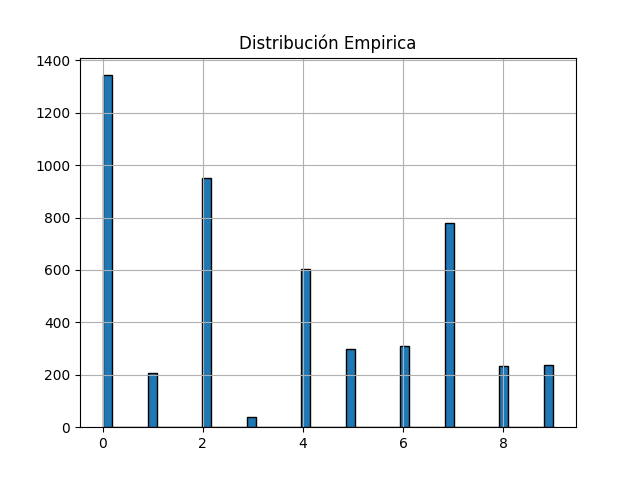
\includegraphics[width=0.7\textwidth]{histograma_empirica.png}
\captionof{figure}{Histograma para la distribución empirica discreta obtenida.}

\end{center}


\end{document}